% Options for packages loaded elsewhere
% Options for packages loaded elsewhere
\PassOptionsToPackage{unicode}{hyperref}
\PassOptionsToPackage{hyphens}{url}
\PassOptionsToPackage{dvipsnames,svgnames,x11names}{xcolor}
%
\documentclass[
  aps,
  pra,
  reprint,
  superscriptaddress]{revtex4-2}
\usepackage{xcolor}
\usepackage{amsmath,amssymb}
\setcounter{secnumdepth}{5}
\usepackage{iftex}
\ifPDFTeX
  \usepackage[T1]{fontenc}
  \usepackage[utf8]{inputenc}
  \usepackage{textcomp} % provide euro and other symbols
\else % if luatex or xetex
  \usepackage{unicode-math} % this also loads fontspec
  \defaultfontfeatures{Scale=MatchLowercase}
  \defaultfontfeatures[\rmfamily]{Ligatures=TeX,Scale=1}
\fi
\usepackage{lmodern}
\ifPDFTeX\else
  % xetex/luatex font selection
\fi
% Use upquote if available, for straight quotes in verbatim environments
\IfFileExists{upquote.sty}{\usepackage{upquote}}{}
\IfFileExists{microtype.sty}{% use microtype if available
  \usepackage[]{microtype}
  \UseMicrotypeSet[protrusion]{basicmath} % disable protrusion for tt fonts
}{}
\makeatletter
\@ifundefined{KOMAClassName}{% if non-KOMA class
  \IfFileExists{parskip.sty}{%
    \usepackage{parskip}
  }{% else
    \setlength{\parindent}{0pt}
    \setlength{\parskip}{6pt plus 2pt minus 1pt}}
}{% if KOMA class
  \KOMAoptions{parskip=half}}
\makeatother
% Make \paragraph and \subparagraph free-standing
\makeatletter
\ifx\paragraph\undefined\else
  \let\oldparagraph\paragraph
  \renewcommand{\paragraph}{
    \@ifstar
      \xxxParagraphStar
      \xxxParagraphNoStar
  }
  \newcommand{\xxxParagraphStar}[1]{\oldparagraph*{#1}\mbox{}}
  \newcommand{\xxxParagraphNoStar}[1]{\oldparagraph{#1}\mbox{}}
\fi
\ifx\subparagraph\undefined\else
  \let\oldsubparagraph\subparagraph
  \renewcommand{\subparagraph}{
    \@ifstar
      \xxxSubParagraphStar
      \xxxSubParagraphNoStar
  }
  \newcommand{\xxxSubParagraphStar}[1]{\oldsubparagraph*{#1}\mbox{}}
  \newcommand{\xxxSubParagraphNoStar}[1]{\oldsubparagraph{#1}\mbox{}}
\fi
\makeatother

\usepackage{color}
\usepackage{fancyvrb}
\newcommand{\VerbBar}{|}
\newcommand{\VERB}{\Verb[commandchars=\\\{\}]}
\DefineVerbatimEnvironment{Highlighting}{Verbatim}{commandchars=\\\{\}}
% Add ',fontsize=\small' for more characters per line
\usepackage{framed}
\definecolor{shadecolor}{RGB}{241,243,245}
\newenvironment{Shaded}{\begin{snugshade}}{\end{snugshade}}
\newcommand{\AlertTok}[1]{\textcolor[rgb]{0.68,0.00,0.00}{#1}}
\newcommand{\AnnotationTok}[1]{\textcolor[rgb]{0.37,0.37,0.37}{#1}}
\newcommand{\AttributeTok}[1]{\textcolor[rgb]{0.40,0.45,0.13}{#1}}
\newcommand{\BaseNTok}[1]{\textcolor[rgb]{0.68,0.00,0.00}{#1}}
\newcommand{\BuiltInTok}[1]{\textcolor[rgb]{0.00,0.23,0.31}{#1}}
\newcommand{\CharTok}[1]{\textcolor[rgb]{0.13,0.47,0.30}{#1}}
\newcommand{\CommentTok}[1]{\textcolor[rgb]{0.37,0.37,0.37}{#1}}
\newcommand{\CommentVarTok}[1]{\textcolor[rgb]{0.37,0.37,0.37}{\textit{#1}}}
\newcommand{\ConstantTok}[1]{\textcolor[rgb]{0.56,0.35,0.01}{#1}}
\newcommand{\ControlFlowTok}[1]{\textcolor[rgb]{0.00,0.23,0.31}{\textbf{#1}}}
\newcommand{\DataTypeTok}[1]{\textcolor[rgb]{0.68,0.00,0.00}{#1}}
\newcommand{\DecValTok}[1]{\textcolor[rgb]{0.68,0.00,0.00}{#1}}
\newcommand{\DocumentationTok}[1]{\textcolor[rgb]{0.37,0.37,0.37}{\textit{#1}}}
\newcommand{\ErrorTok}[1]{\textcolor[rgb]{0.68,0.00,0.00}{#1}}
\newcommand{\ExtensionTok}[1]{\textcolor[rgb]{0.00,0.23,0.31}{#1}}
\newcommand{\FloatTok}[1]{\textcolor[rgb]{0.68,0.00,0.00}{#1}}
\newcommand{\FunctionTok}[1]{\textcolor[rgb]{0.28,0.35,0.67}{#1}}
\newcommand{\ImportTok}[1]{\textcolor[rgb]{0.00,0.46,0.62}{#1}}
\newcommand{\InformationTok}[1]{\textcolor[rgb]{0.37,0.37,0.37}{#1}}
\newcommand{\KeywordTok}[1]{\textcolor[rgb]{0.00,0.23,0.31}{\textbf{#1}}}
\newcommand{\NormalTok}[1]{\textcolor[rgb]{0.00,0.23,0.31}{#1}}
\newcommand{\OperatorTok}[1]{\textcolor[rgb]{0.37,0.37,0.37}{#1}}
\newcommand{\OtherTok}[1]{\textcolor[rgb]{0.00,0.23,0.31}{#1}}
\newcommand{\PreprocessorTok}[1]{\textcolor[rgb]{0.68,0.00,0.00}{#1}}
\newcommand{\RegionMarkerTok}[1]{\textcolor[rgb]{0.00,0.23,0.31}{#1}}
\newcommand{\SpecialCharTok}[1]{\textcolor[rgb]{0.37,0.37,0.37}{#1}}
\newcommand{\SpecialStringTok}[1]{\textcolor[rgb]{0.13,0.47,0.30}{#1}}
\newcommand{\StringTok}[1]{\textcolor[rgb]{0.13,0.47,0.30}{#1}}
\newcommand{\VariableTok}[1]{\textcolor[rgb]{0.07,0.07,0.07}{#1}}
\newcommand{\VerbatimStringTok}[1]{\textcolor[rgb]{0.13,0.47,0.30}{#1}}
\newcommand{\WarningTok}[1]{\textcolor[rgb]{0.37,0.37,0.37}{\textit{#1}}}

\usepackage{longtable,booktabs,array}
\newcounter{none} % for unnumbered tables
\usepackage{calc} % for calculating minipage widths
% Correct order of tables after \paragraph or \subparagraph
\usepackage{etoolbox}
\makeatletter
\patchcmd\longtable{\par}{\if@noskipsec\mbox{}\fi\par}{}{}
\makeatother
% Allow footnotes in longtable head/foot
\IfFileExists{footnotehyper.sty}{\usepackage{footnotehyper}}{\usepackage{footnote}}
\makesavenoteenv{longtable}
\usepackage{graphicx}
\makeatletter
\newsavebox\pandoc@box
\newcommand*\pandocbounded[1]{% scales image to fit in text height/width
  \sbox\pandoc@box{#1}%
  \Gscale@div\@tempa{\textheight}{\dimexpr\ht\pandoc@box+\dp\pandoc@box\relax}%
  \Gscale@div\@tempb{\linewidth}{\wd\pandoc@box}%
  \ifdim\@tempb\p@<\@tempa\p@\let\@tempa\@tempb\fi% select the smaller of both
  \ifdim\@tempa\p@<\p@\scalebox{\@tempa}{\usebox\pandoc@box}%
  \else\usebox{\pandoc@box}%
  \fi%
}
% Set default figure placement to htbp
\def\fps@figure{htbp}
\makeatother





\setlength{\emergencystretch}{3em} % prevent overfull lines

\providecommand{\tightlist}{%
  \setlength{\itemsep}{0pt}\setlength{\parskip}{0pt}}



 
\usepackage[]{natbib}
\bibliographystyle{apsrev4-2}


% caption (via ltcaption) defines a longtable* environment, and RevTeX later tries to
% \newenvironment its own in begindocument/before, which fails. Remove caption's
% version just before RevTeX installs its own.
\AddToHook{begindocument/before}[revtex-fix]{%
  \expandafter\let\csname longtable*\endcsname\relax
  \expandafter\let\csname endlongtable*\endcsname\relax
}
\DeclareHookRule{begindocument/before}{revtex-fix}{before}{revtex4-2}
\makeatletter
\@ifpackageloaded{caption}{}{\usepackage{caption}}
\AtBeginDocument{%
\ifdefined\contentsname
  \renewcommand*\contentsname{Table of contents}
\else
  \newcommand\contentsname{Table of contents}
\fi
\ifdefined\listfigurename
  \renewcommand*\listfigurename{List of Figures}
\else
  \newcommand\listfigurename{List of Figures}
\fi
\ifdefined\listtablename
  \renewcommand*\listtablename{List of Tables}
\else
  \newcommand\listtablename{List of Tables}
\fi
\ifdefined\figurename
  \renewcommand*\figurename{Figure}
\else
  \newcommand\figurename{Figure}
\fi
\ifdefined\tablename
  \renewcommand*\tablename{Table}
\else
  \newcommand\tablename{Table}
\fi
}
\@ifpackageloaded{float}{}{\usepackage{float}}
\floatstyle{ruled}
\@ifundefined{c@chapter}{\newfloat{codelisting}{h}{lop}}{\newfloat{codelisting}{h}{lop}[chapter]}
\floatname{codelisting}{Listing}
\newcommand*\listoflistings{\listof{codelisting}{List of Listings}}
\makeatother
\makeatletter
\makeatother
\makeatletter
\@ifpackageloaded{caption}{}{\usepackage{caption}}
\@ifpackageloaded{subcaption}{}{\usepackage{subcaption}}
\makeatother
% STIX Two text and math fonts from _fonts/ (requires lualatex or xelatex).
\usepackage{unicode-math}
\setmainfont{STIXTwoText}[
  Path = _fonts/,
  Extension = .ttf,
  UprightFont = *-Regular,
  ItalicFont = *-Italic,
  BoldFont = *-Bold,
  BoldItalicFont = *-BoldItalic,
]
\setmathfont{STIXTwoMath-Regular.otf}[Path = _fonts/]
\usepackage{bookmark}
\IfFileExists{xurl.sty}{\usepackage{xurl}}{} % add URL line breaks if available
\urlstyle{same}
\hypersetup{
  pdftitle={A Quarto manuscript template for RevTeX},
  colorlinks=true,
  linkcolor={blue},
  filecolor={Maroon},
  citecolor={Blue},
  urlcolor={Blue},
  pdfcreator={LaTeX via pandoc}}



\begin{document}
\title{A Quarto manuscript template for RevTeX}
\author{First Author}
\email{first.author@example.org}
\affiliation{Department of Examples, First University}
\author{Second Author}
\affiliation{Department of Examples, First University}
\affiliation{Institute of Templates, Second University}
\begin{abstract}
This is a placeholder abstract. The document demonstrates the features
of a Quarto manuscript project that renders a RevTeX PDF: author and
affiliation metadata, numbered sections and equations, cross-references,
citations, and figures generated from Python code.
\end{abstract}
\maketitle


\section{Workflow}\label{sec-workflow}

This section documents how the manuscript is built and should be removed
before submission. The source is the Quarto file \texttt{index.qmd}, and
\texttt{\_quarto.yml} configures a Quarto \emph{manuscript} project that
renders HTML, Word, JATS and a RevTeX PDF from that single source.

\subsection{Building}\label{building}

Render all formats, or only the PDF, with

\begin{Shaded}
\begin{Highlighting}[]
\ExtensionTok{quarto}\NormalTok{ render}
\ExtensionTok{quarto}\NormalTok{ render index.qmd }\AttributeTok{{-}{-}to}\NormalTok{ pdf}
\end{Highlighting}
\end{Shaded}

Output is written to \texttt{\_manuscript/}. Because
\texttt{freeze:\ true} is set, a project-wide render reuses stored code
output; rendering \texttt{index.qmd} explicitly re-executes the Python
chunks. Use \texttt{quarto\ preview} for live reloading while writing.

\subsection{RevTeX setup}\label{revtex-setup}

The PDF uses \texttt{documentclass:\ revtex4-2} with the options
\texttt{aps,\ pra,\ reprint,\ superscriptaddress}; change \texttt{pra}
to target another journal, or \texttt{reprint} to \texttt{preprint} for
a single-column draft. The folder \texttt{\_revtex/} holds the glue
between Quarto and RevTeX. The file \texttt{before-body.tex} emits
\texttt{\textbackslash{}title}, \texttt{\textbackslash{}author},
\texttt{\textbackslash{}affiliation}, \texttt{\textbackslash{}email} and
the abstract after \texttt{\textbackslash{}begin\{document\}}, as RevTeX
requires. The file \texttt{preamble.tex} resolves a \texttt{longtable*}
clash with the \texttt{caption} package. The generated LaTeX is kept in
\texttt{\_manuscript/\_tex/} for journal submission.

\subsection{Fonts}\label{fonts}

Text and mathematics are set in STIX Two in both the PDF and the HTML
output. The font files are in \texttt{\_fonts/}, and they are switched
on by \texttt{stix:\ true} in \texttt{\_quarto.yml}; set it to
\texttt{false} to use the default fonts. The filter
\texttt{\_fonts/stix.lua} loads the fonts in the PDF preamble and, for
HTML, tells MathJax 4 to use its STIX Two math font.

\subsection{Plots}\label{sec-plots}

The first code chunk in this file loads the local package
\texttt{revtexplot}, which styles matplotlib figures to match the PDF.
It is switched on by \texttt{plot-style:\ true} in
\texttt{\_quarto.yml}; set it to \texttt{false} for matplotlib's
defaults. Figures are one column wide by default and use 8 pt text, the
size of \texttt{\textbackslash{}footnotesize}, in STIX Two (or Computer
Modern with \texttt{stix:\ false}). They are saved at exactly their set
size, so the text in them matches the captions. The package provides
these sizes:

\begin{itemize}
\tightlist
\item
  \texttt{rp.COLUMN}: one column, 3.40 × 2.10 in (the default)
\item
  \texttt{rp.WIDE}: both columns, 7.06 × 2.35 in
\item
  \texttt{rp.figsize(width,\ aspect)}: \texttt{width} is
  \texttt{"column"}, \texttt{"wide"} or inches, and \texttt{aspect} is
  height / width
\end{itemize}

For example, \texttt{plt.subplots(figsize=rp.figsize("column",\ 1))}
gives a square one-column figure.

\subsection{Writing}\label{writing}

Authors, affiliations, e-mail addresses and the abstract are set in the
YAML header. Sections, equations and figures get labels with the
prefixes \texttt{sec-}, \texttt{eq-} and \texttt{fig-}, and are
referenced as \texttt{@sec-methods}, \texttt{@eq-gaussian} or
\texttt{@fig-example}. A displayed equation is labelled by appending
\texttt{\{\#eq-name\}} after its closing \texttt{\$\$}. Citations use
keys from \texttt{references.bib}, e.g.~\texttt{{[}@knuth1984{]}}, and
are formatted by BibTeX with the \texttt{apsrev4-2} style. Figures are
produced by Python chunks whose \texttt{label} and \texttt{fig-cap}
options set the reference and caption; see Section~\ref{sec-results} for
an example.

\subsection{Wide figures and
equations}\label{wide-figures-and-equations}

In the two-column \texttt{reprint} layout, a figure spans both columns
when it uses RevTeX's \texttt{figure*} environment. For a Python chunk,
add the options

\begin{Shaded}
\begin{Highlighting}[]
\CommentTok{\#| fig{-}env: "figure*"}
\CommentTok{\#| fig{-}pos: "t"}
\end{Highlighting}
\end{Shaded}

and create the figure with \texttt{plt.subplots(figsize=rp.WIDE)} (see
Section~\ref{sec-plots}). For an image file, write

\begin{Shaded}
\begin{Highlighting}[]
\AlertTok{![Caption.](figures/wide.pdf)}\NormalTok{\{\#fig{-}wide}
\NormalTok{  fig{-}env="figure*" fig{-}pos="t"\}}
\end{Highlighting}
\end{Shaded}

Wide figures float to the top of a following page. Always set
\texttt{fig-pos:\ "t"}: Quarto places chunk figures with
\texttt{{[}H{]}} by default, which makes a \texttt{figure*} vanish from
the PDF. Do not use \texttt{column:\ page}; it loads the
\texttt{sidenotes} package, which stops every \texttt{figure*} from
spanning both columns.

A long equation is set across both columns by wrapping it in RevTeX's
\texttt{widetext} environment with raw LaTeX blocks:

\begin{Shaded}
\begin{Highlighting}[]
\InformationTok{\textasciigrave{}\textasciigrave{}\textasciigrave{}\{=latex\}}
\InformationTok{\textbackslash{}begin\{widetext\}}
\InformationTok{\textasciigrave{}\textasciigrave{}\textasciigrave{}}
\NormalTok{$$}
\NormalTok{E = \textbackslash{}sum\_n a\_n x\^{}n + \textbackslash{}dots}
\NormalTok{$$ \{\#eq{-}wide\}}
\InformationTok{\textasciigrave{}\textasciigrave{}\textasciigrave{}\{=latex\}}
\InformationTok{\textbackslash{}end\{widetext\}}
\InformationTok{\textasciigrave{}\textasciigrave{}\textasciigrave{}}
\end{Highlighting}
\end{Shaded}

Labels and cross-references work as usual. The HTML output ignores
\texttt{fig-env}, \texttt{fig-pos} and the raw LaTeX, so both render
normally there.

\section{Introduction}\label{introduction}

This is placeholder text for the introduction. Literate programming
\citep{knuth1984} advocates weaving code and prose into a single
document, an idea that Quarto applies to scientific manuscripts. The
typesetting itself is done by TeX \citep{knuth1986} and LaTeX
\citep{lamport1994}. Multiple references can be cited together
\citep{knuth1984, lamport1994}.

\section{Methods}\label{sec-methods}

\subsection{Inline and displayed
mathematics}\label{inline-and-displayed-mathematics}

Inline mathematics is written between single dollar signs, as in
\(e^{i\pi} + 1 = 0\). Displayed equations are written between double
dollar signs and numbered when given a label, as for the Gaussian
integral \begin{equation}\protect\phantomsection\label{eq-gaussian}{
\int_{-\infty}^{\infty} e^{-a x^2}\, dx = \sqrt{\frac{\pi}{a}},
\qquad a > 0.
}\end{equation}

\subsection{Multi-line equations}\label{multi-line-equations}

Long expressions can be split with an \texttt{aligned} environment
inside a single labelled equation,
\begin{equation}\protect\phantomsection\label{eq-taylor}{
\begin{aligned}
f(x) &= \sum_{n=0}^{\infty} \frac{f^{(n)}(x_0)}{n!} (x - x_0)^n \\
     &= f(x_0) + f'(x_0)(x - x_0) + \mathcal{O}\big((x - x_0)^2\big).
\end{aligned}
}\end{equation}

\subsection{Cross-references}\label{cross-references}

Equations are referenced as Equation~\ref{eq-gaussian} and
Equation~\ref{eq-taylor}, sections as Section~\ref{sec-results}, and
figures as Figure~\ref{fig-example}. The numbers are assigned
automatically in every output format.

\section{Results}\label{sec-results}

Figure~\ref{fig-example} is generated by the Python code chunk embedded
in the source file. It shows the damped oscillation
\begin{equation}\protect\phantomsection\label{eq-damped}{
f(t) = e^{-\gamma t} \cos(\omega t).
}\end{equation} for three values of the damping rate \(\gamma\).

\begin{figure}[H]

\centering{

\pandocbounded{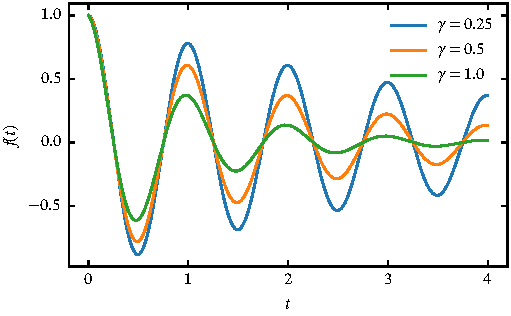
\includegraphics[keepaspectratio]{index_files/figure-pdf/fig-example-output-1.pdf}}

}

\caption{\label{fig-example}Damped oscillations for three values of the
damping rate \(\gamma\), with \(\omega = 2\pi\).}

\end{figure}%

Figure~\ref{fig-wide} spans both columns and shows each damping rate in
its own panel.

\begin{figure*}[t]

\centering{

\pandocbounded{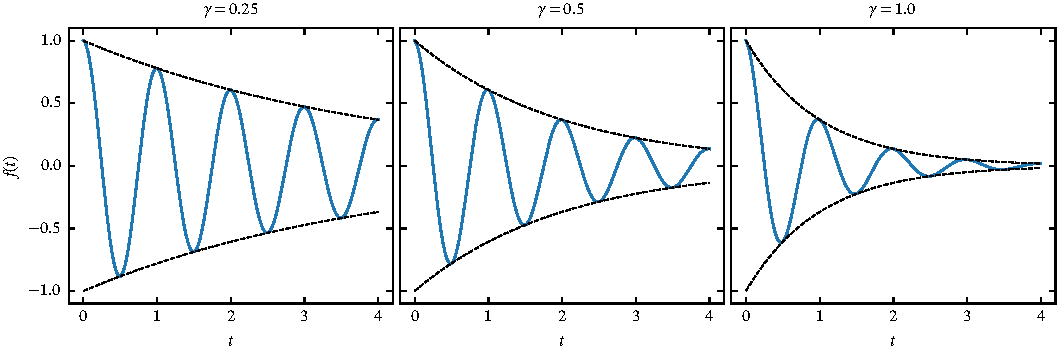
\includegraphics[keepaspectratio]{index_files/figure-pdf/fig-wide-output-1.pdf}}

}

\caption{\label{fig-wide}The oscillations of Figure~\ref{fig-example}
with their envelopes \(\pm e^{-\gamma t}\) (dashed).}

\end{figure*}%

\section{Conclusion}\label{conclusion}

This is placeholder text for the conclusion. Replace the contents of
this file with your own manuscript, keeping Section~\ref{sec-workflow}
as a reference until submission.


\bibliography{references.bib}



\end{document}
